\section{Predictive Modeling – Linear Regression and Rainfall Forecasting}

Predictive modeling is a fundamental aspect of advanced data analytics. It involves using statistical techniques to forecast future values based on historical data. In the context of climate science, predictive models can be used to anticipate key environmental variables such as temperature, humidity, and precipitation.

One of the most commonly used predictive methods is regression analysis, which quantifies the relationship between a dependent variable and one or more independent variables. For example, we might use wind speed and humidity levels to predict rainfall amounts. By fitting a mathematical model to observed data, we can make informed projections about future conditions.

Predictive modeling in climate data offers several key benefits:
\begin{itemize}
  \item \textbf{Forecasting:} Provides estimations of future climate conditions, such as rainfall trends or temperature fluctuations.
  \item \textbf{Planning and Preparedness:} Supports agricultural planning, disaster risk reduction, and water resource management.
  \item \textbf{Insight into Variable Interactions:} Helps understand how different climatic factors influence one another.
\end{itemize}

In this chapter, we will:
\begin{itemize}
  \item Apply linear regression to model rainfall based on other climatic parameters.
  \item Interpret the model coefficients and assess the quality of predictions.
  \item Evaluate the model’s performance using statistical metrics.
\end{itemize}

This analytical approach enables a data-driven understanding of weather behavior, enhancing our ability to predict and prepare for changing climate scenarios.

\subsection*{Linear Regression Model Preparation and Evaluation}

In this section, we will build a linear regression model to predict precipitation based on two climatic parameters: temperature and humidity. This approach helps us understand how these variables contribute to rainfall patterns and allows us to make future predictions.

\subsubsection*{Step 1: Selecting the Variables}

We begin by selecting relevant variables from our dataset:

\begin{verbatim}
model_data <- climate_data %>%
  select(Temp_2m, Precip, Humidity_2m)
\end{verbatim}

\subsubsection*{Step 2: Fitting the Linear Regression Model}

We now fit a multiple linear regression model. The formula for the model is as follows:

\[
\text{Precipitation} = \beta_0 + \beta_1 \cdot \text{Temp\_2m} + \beta_2 \cdot \text{Humidity\_2m} + \epsilon
\]

Here, \(\beta_0\) is the intercept, \(\beta_1\) and \(\beta_2\) are the coefficients, and \(\epsilon\) represents the error term.

\begin{verbatim}
model <- lm(Precip ~ Temp_2m + Humidity_2m, data = model_data)
summary(model)
\end{verbatim}

The \texttt{summary(model)} function provides details about the coefficients and statistical significance of each variable, which help interpret how temperature and humidity influence precipitation.

\subsubsection*{Step 3: Making Predictions}

Using the fitted model, we generate predicted precipitation values:

\begin{verbatim}
predictions <- predict(model, newdata = model_data)
\end{verbatim}

% Figure here---------------------------
\begin{figure}[h]
\centering
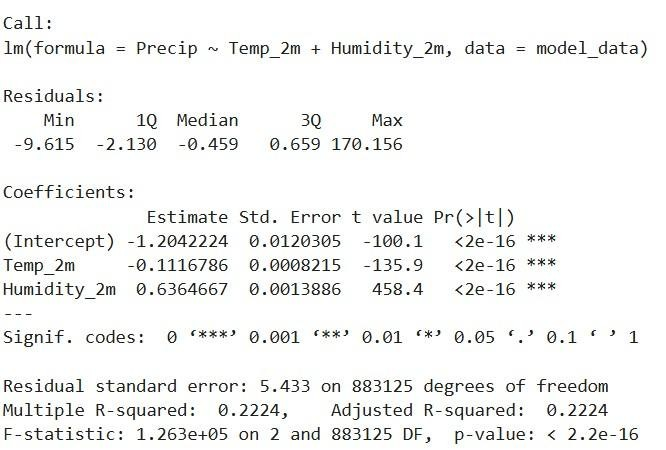
\includegraphics[width=0.6\textwidth]{figures/regression.jpg}
\caption{Model summary}
\end{figure}

\subsubsection*{Step 4: Model Evaluation}

To assess the model’s performance, we calculate:

\begin{itemize}
  \item \textbf{R-squared (R\(^2\))}: Measures how well the predictors explain the variance in the target variable. Values closer to 1 indicate a better fit.
  \item \textbf{Mean Squared Error (MSE)}: Measures the average squared difference between actual and predicted values. Lower MSE indicates better accuracy.
\end{itemize}

\begin{verbatim}
r_squared <- summary(model)$r.squared
mse <- mean((predictions - model_data$Precip)^2)

actual_avg <- mean(model_data$Precip)
predicted_avg <- mean(predictions)

cat("R-squared:", r_squared, "\n")
cat("Mean Squared Error (MSE):", mse, "\n")
cat("Actual Average Precipitation:", actual_avg, "\n")
cat("Predicted Average Precipitation:", predicted_avg, "\n")
\end{verbatim}

% Figure here-----------------------------
\begin{figure}[h]
\centering
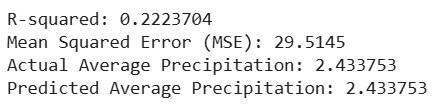
\includegraphics[width=0.5\textwidth]{figures/r_square.jpg}
\caption{Model evaluation metrics}
\end{figure}

\subsubsection*{Step 5: Visualizing Model Performance}

\textbf{Actual vs Predicted Plot:} This scatter plot compares the real precipitation values against the model’s predictions. The red line (y = x) indicates perfect prediction. Points close to this line show accurate predictions.

\begin{verbatim}
plot(model_data$Precip, predictions,
     xlab = "Actual Precipitation",
     ylab = "Predicted Precipitation",
     main = "Actual vs Predicted Precipitation")
abline(0, 1, col = "red")
\end{verbatim}

\textbf{Residual Plot:} This shows the residuals (errors) from the predictions. Ideally, residuals should be randomly scattered around zero. Patterns in residuals could suggest issues with the model fit.

\begin{verbatim}
residuals <- model$residuals
plot(residuals, main = "Residuals",
     ylab = "Residuals", xlab = "Index")
abline(h = 0, col = "red")
\end{verbatim}

% Figure here----------------------------
\begin{figure}[h]
\centering
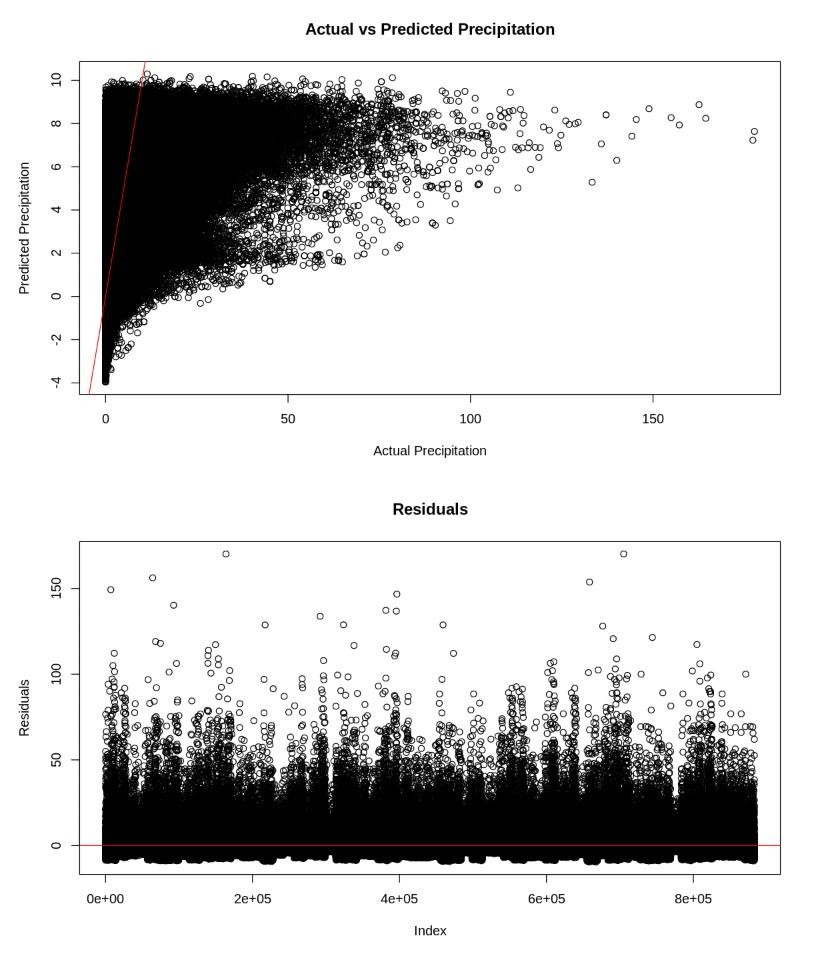
\includegraphics[width=0.5\textwidth]{figures/pred_residual.jpg}
\caption{Actual vs Predicted Plot and Residual Plot}
\end{figure}

\subsection*{Conclusion}

Through this exercise, we’ve seen how a simple regression model can be applied to climate data. We evaluated the model’s effectiveness using statistical metrics and visualizations, which are essential for interpreting the reliability and accuracy of predictions. As you explore more advanced models, this foundational approach will remain a critical tool for climate data analysis.
\clearpage

\subsection*{Predicting the Likelihood of Rainfall Based on Temperature and Humidity}

In this section, we’ll build a logistic regression model to predict whether rainfall will occur, using temperature and humidity as predictors. Instead of predicting how much rain will fall, we simplify the problem into a binary classification: Did it rain or not?

\subsubsection*{Step 1: Preparing the Data}

We start by creating a new variable in our dataset called \textit{Rain Occurrence}. This variable holds:

\begin{itemize}
  \item 1 if precipitation is greater than 0mm (indicating it rained)
  \item 0 otherwise (indicating no rain).
\end{itemize}

\begin{verbatim}
rain_data <- climate_data %>%
  mutate(Rain_Occurrence = ifelse(Precip > 0, 1, 0)) %>%
  select(Temp_2m, Humidity_2m, Rain_Occurrence)
\end{verbatim}

\subsubsection*{Step 2: Splitting the Dataset}

We divide our data into two parts:

\begin{itemize}
  \item \textbf{Training Set (80\%):} Used to train the model.
  \item \textbf{Testing Set (20\%):} Used to evaluate model performance.
\end{itemize}

\begin{verbatim}
set.seed(123)
train_index <- createDataPartition(rain_data$Rain_Occurrence, p = 0.8, 
list = FALSE)
train_data <- rain_data[train_index, ]
test_data <- rain_data[-train_index, ]
\end{verbatim}

\subsubsection*{Step 3: Standardizing the Features}

Before training, we standardize the temperature and humidity values to have a mean of 0 and a standard deviation of 1. This ensures that all features contribute equally to the model.

\begin{verbatim}
preprocess <- preProcess(train_data[, c("Temp_2m", "Humidity_2m")], 
method = c("center", "scale"))
train_data[, c("Temp_2m", "Humidity_2m")] <- predict(preprocess, 
train_data[, c("Temp_2m", "Humidity_2m")])
test_data[, c("Temp_2m", "Humidity_2m")] <- predict(preprocess, 
test_data[, c("Temp_2m", "Humidity_2m")])
\end{verbatim}

\subsubsection*{Step 4: Training the Logistic Regression Model}

We now fit a logistic regression model. This model estimates the probability of rain occurring based on the input temperature and humidity.

\begin{verbatim}
logistic_model <- glm(Rain_Occurrence ~ Temp_2m + Humidity_2m,
                      data = train_data, family = "binomial")
\end{verbatim}

\subsubsection*{Step 5: Making Predictions}

Once the model is trained, we make predictions on the test data:

\begin{itemize}
  \item Predicted Probability: the probability that rain will occur.
  \item Predicted Class: the classification (1 = rain, 0 = no rain) based on a threshold of 0.5.
\end{itemize}

\begin{verbatim}
test_data$Predicted_Prob <- predict(logistic_model, test_data,
type = "response")
test_data$Predicted_Class <- ifelse(test_data$Predicted_Prob > 0.5, 1, 0)
\end{verbatim}

\subsubsection*{Step 6: Evaluating the Model}

To assess the model’s effectiveness, we use a confusion matrix and compute several metrics:

\begin{itemize}
  \item \textbf{Accuracy:} Proportion of total correct predictions.
  \item \textbf{Precision:} Out of the times the model predicted rain, how often it was correct.
  \item \textbf{Recall (Sensitivity):} Out of the actual rainy instances, how many were correctly predicted.
  \item \textbf{F1-score:} Harmonic mean of precision and recall.
\end{itemize}

\begin{verbatim}
conf_matrix <- confusionMatrix(as.factor(test_data$Predicted_Class),
                               as.factor(test_data$Rain_Occurrence))

accuracy <- conf_matrix$overall["Accuracy"]
precision <- conf_matrix$byClass["Precision"]
recall <- conf_matrix$byClass["Recall"]
f1_score <- 2 * ((precision * recall) / (precision + recall))

cat("Accuracy:", accuracy, "\n")
cat("Precision:", precision, "\n")
cat("Recall:", recall, "\n")
cat("F1 Score:", f1_score, "\n")
\end{verbatim}

% Figure here----------------------------
\begin{figure}[h]
\centering
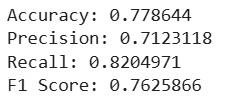
\includegraphics[width=0.3\textwidth]{figures/eval_metrics.jpg}
\caption{Evaluation metrics}
\end{figure}

\subsubsection*{Step 7: Visualizing Performance with the ROC Curve}

The ROC (Receiver Operating Characteristic) curve helps us visualize how well the model distinguishes between rainy and non-rainy days. The curve plots:

\begin{itemize}
  \item True Positive Rate (Recall) on the y-axis,
  \item False Positive Rate on the x-axis.
\end{itemize}

A curve closer to the top-left corner indicates better performance.

\begin{verbatim}
roc_curve <- roc(test_data$Rain_Occurrence, test_data$Predicted_Prob)
ggroc(roc_curve) +
labs(
  title = "ROC Curve", 
  x = "False Positive Rate", y = "True Positive Rate") +
theme_minimal()
\end{verbatim}

% Figure here--------------------------
\begin{figure}[h]
\centering
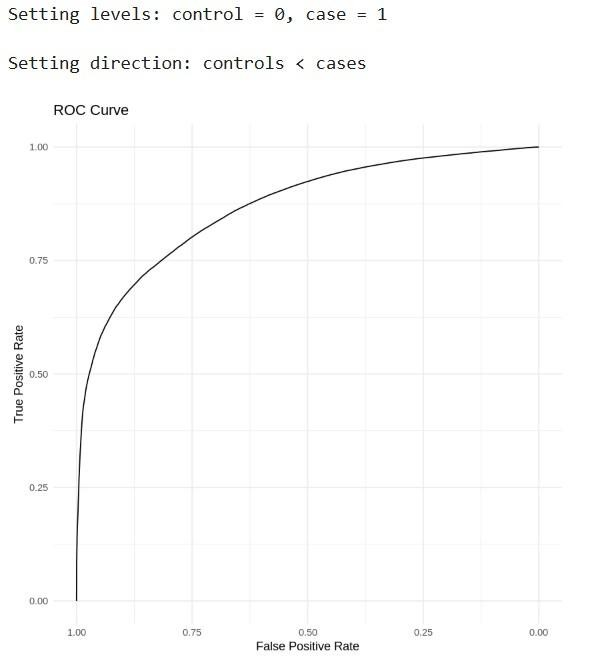
\includegraphics[width=0.5\textwidth]{figures/ROC.jpg}
\caption{ROC curve}
\end{figure}

\subsection*{Conclusion}

This logistic regression model gives us a practical tool to estimate the probability of rainfall using just temperature and humidity. While the model is simple, it introduces key classification concepts and serves as a foundation for more complex predictive techniques in climate analytics.
